\documentclass{article}
\usepackage{amsmath}
\usepackage{geometry}
\usepackage{pdfpages}
\usepackage{graphicx}
\graphicspath{{./}}
\geometry{letterpaper, portrait, margin=1in}

\title{Math 252 Homework\\
\large Sections 4.2 \& 4.3}
\date{2016/04/03}
\author{Solomon Greenberg}


\begin{document}
    \pagenumbering{gobble}
    \maketitle
    \newpage
    \pagenumbering{arabic}

    \section*{Chapter 4.2}
    \paragraph*{1:\\}
        An absolute minimum is a point at the lowest value that a graph reaches over an interval that, if the interval is open, does not include the limits of the interval. A relative minimum is any point that has a lesser value than the the points directly to the left or right of it.

    \paragraph*{5:\\}
        Local minima: (2, 2), (5, 3) \\
        Local maxima: (4, 5) \\
        Absolute minima: (0, 2), (2, 2) \\
        Absolute maxima: (4, 5) \\

    \paragraph*{11:\\} 
        a:\\ 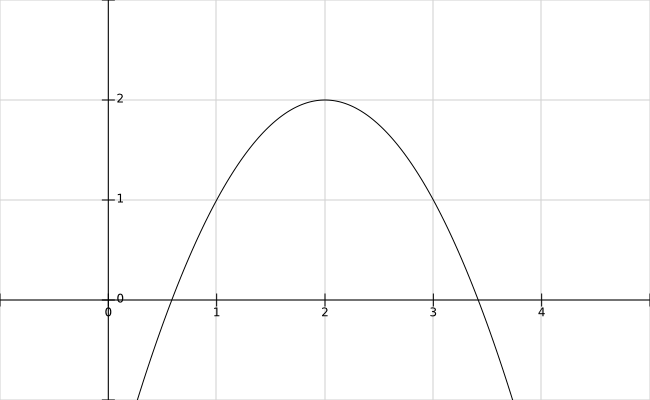
\includegraphics[scale=.333]{graph11a.png}\\\\
        b:\\ 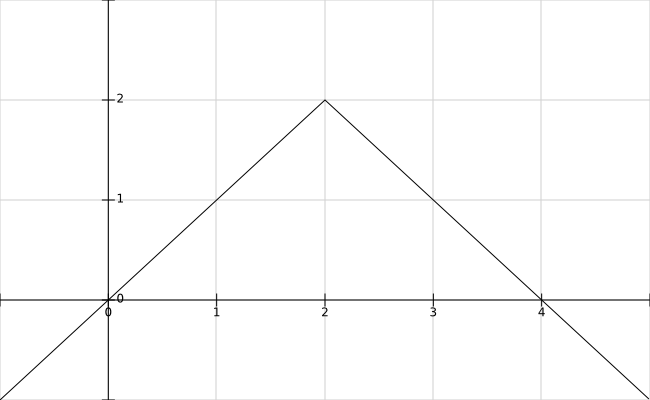
\includegraphics[scale=.333]{graph11b.png}\\\\
        c:\\ 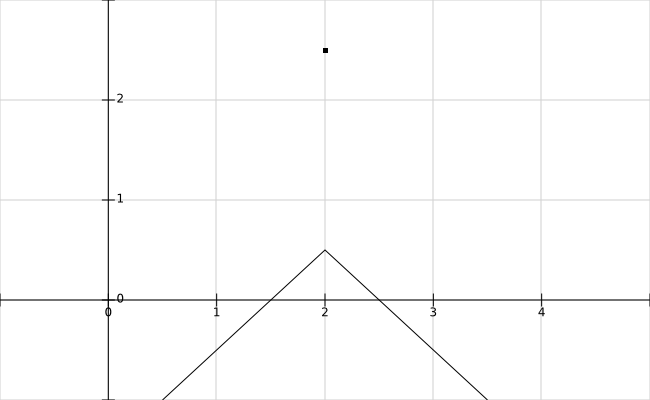
\includegraphics[scale=.333]{graph11c.png}\\\\

    \paragraph*{29:\\}
        Note: Used calculator (Ti-$n$spire CX CAS) to find x-intercepts of \begin {math} f'(y) \end {math} \\
        Critical numbers at \begin{math} x=\{0, 2\} \end {math}\\ 

    \paragraph*{35:\\}
        Note: used calculator (Ti-$n$spire CX CAS) to find x-intercepts of \begin{math} f'(\theta) \end{math} \\
        Critical numbers at \begin{math} \theta=\{2 \cdot n \cdot \pi, n \cdot \pi\} \end{math} \\

    \paragraph*{43:\\}
        Absolute maxima: $(-1, 8)$\\ Absolute minima: $(2, -18)$\\

    \paragraph*{51:\\}
        Absolute maxima: $(1, \ln(3))$\\ Absolute minima: $(1, \ln(1.75))$\\

    \paragraph*{59:\\}
        $f(x) = x\cdot \sqrt{x-x^2}$\\
        a: No absolute min/max as function is consistantly concave down and on an open interval.\\
        b: Likewise

    \paragraph*{61:\\}
        $V = 999.87 - 0.06426T - 0.0085043T^2 - 0.0000679T^3$\\
        Max.\ density at $x = 208.614$
    
    \section*{Chapter 4.3}
    \paragraph*{2:\\}
        Concave upward:   $(2, 4), (16/3, 8)$\\
        Concave downward: $(0, 2), (4, 16/3)$\\

        \paragraph{6:\\}

        
    



\end{document}

